\documentclass{article}

% Use a NeurIPS-compatible style if available; otherwise plain article
\usepackage[utf8]{inputenc}
\usepackage[T1]{fontenc}
\usepackage{hyperref}
\usepackage{url}
\usepackage{booktabs}
\usepackage{amsfonts}
\usepackage{amsmath}
\usepackage{amssymb}
\usepackage{graphicx}
\usepackage{xcolor}
\usepackage{algorithm}
\usepackage{algorithmic}
\usepackage{microtype}
\usepackage{enumitem}
\usepackage[margin=1in]{geometry}

\title{Agent RL for Diffusion Language Models:\\Multi-Turn Tool-Calling via Segment-Aware Policy Optimization}

\author{
  Anonymous Authors
}

\date{}

\begin{document}
\maketitle

% ════════════════════════════════════════════════════════════
\begin{abstract}
Recent advances in reinforcement learning (RL) for large language models (LLMs) have enabled multi-turn agent training with tool use, but all existing methods---including RAGEN, SimpleTIR, and RLFactory---assume autoregressive (AR) generation. We present the first framework for training \textbf{multi-turn tool-calling agents} on \textbf{diffusion language models} (dLLMs), which generate text through iterative denoising rather than left-to-right token emission. Our framework addresses three key challenges: (1)~\emph{segment-aware masking} that distinguishes model-generated tokens from environment-injected observations in multi-turn trajectories, (2)~\emph{cross-turn step-map composition} that extends TraceRL's trajectory-aware credit assignment across interaction turns, and (3)~a \emph{turn-by-turn diffusion generation} protocol for tool calling. We evaluate on GSM8K using LLaDA-8B with a calculator tool. All RL variants improve over zero-shot (8.5\%), with standard single-turn RL reaching 18.0\% and agent RL variants reaching 12--20\%. We find that training on observation tokens (without segment masking) yields the strongest agent RL result (20.0\%), and that TraceRL consistently outperforms random masking in the agent setting. Our results demonstrate the feasibility of agent RL for dLLMs while revealing that the value of tool access depends critically on benchmark characteristics.
\end{abstract}

% ════════════════════════════════════════════════════════════
\section{Introduction}

Diffusion language models (dLLMs) have emerged as a promising alternative to autoregressive (AR) LLMs, offering parallel generation, flexible editing, and natural infilling capabilities~\citep{austin2021d3pm, lou2024mdlm, nie2025llada}. Recent work has shown that RL post-training can substantially improve dLLMs' reasoning abilities: TraceRL~\citep{tracerl2025} introduces trajectory-aware credit assignment for masked diffusion models, achieving significant gains on math benchmarks.

Concurrently, the field of LLM agent training has advanced rapidly. Methods like RAGEN~\citep{wang2025ragen}, SimpleTIR~\citep{xue2025simpletir}, and RLFactory~\citep{chai2025rlfactory} enable multi-turn RL training where models learn to use external tools---search engines, code interpreters, calculators---through interaction with environments. However, \textbf{all existing agent RL methods assume autoregressive generation}. No prior work has addressed how to train tool-calling agents on diffusion language models.

This gap is non-trivial. Diffusion LLMs generate text through iterative denoising over the \emph{full} sequence, fundamentally changing how actions are produced, how token-level probabilities are computed, and how gradients flow. Extending agent RL to dLLMs requires solving three technical challenges:

\begin{enumerate}[leftmargin=*,itemsep=2pt]
    \item \textbf{Segment-aware masking.} In multi-turn agent trajectories, model-generated tokens and environment-injected observations are interleaved. Standard diffusion training would mask/train over observation tokens indiscriminately. We introduce a trainable mask that tracks segment boundaries.

    \item \textbf{Cross-turn step-map composition.} TraceRL uses the denoising trajectory (step-map) for credit assignment within a single generation. We extend this across multiple interaction turns, maintaining globally consistent denoising-order information.

    \item \textbf{Turn-by-turn diffusion generation.} Unlike AR models that can simply append tokens, dLLMs must run a complete denoising process for each generation turn, with tool observations injected as frozen context between turns.
\end{enumerate}

We implement these ideas as an extension to the dLLM-RL framework~\citep{tracerl2025} and evaluate on GSM8K~\citep{cobbe2021gsm8k} with a calculator tool. Our experiments reveal several findings:
\begin{itemize}[leftmargin=*,itemsep=2pt]
    \item All RL methods (with or without tools) substantially improve over zero-shot, confirming that RL post-training works for dLLMs on math reasoning.
    \item TraceRL consistently outperforms random masking in the agent setting (14.0\% vs 12.0\%), validating trajectory-aware credit assignment for multi-turn dLLM training.
    \item Surprisingly, training \emph{without} segment-aware masking yields the strongest agent RL result (20.0\% vs 14.0\%), suggesting that observation tokens provide useful learning signal.
    \item Standard single-turn RL (18.0\%) outperforms agent RL with tools (14.0\%) on GSM8K, indicating that tool access does not help when the bottleneck is reasoning setup rather than computation.
\end{itemize}

Our work makes two contributions: (1)~the first complete framework for multi-turn agent RL on diffusion language models, and (2)~an empirical analysis of when tool access helps (or hurts) dLLM agents.

% ════════════════════════════════════════════════════════════
\section{Related Work}

\paragraph{Diffusion Language Models.}
Discrete diffusion models for text generation~\citep{austin2021d3pm, he2022diffusionbert} have evolved into competitive language models. MDLM~\citep{lou2024mdlm} and SEDD~\citep{lou2024sedd} achieve strong perplexity with score-based discrete diffusion. LLaDA~\citep{nie2025llada} scales masked diffusion to 8B parameters, demonstrating competitive performance with AR models. Dream~\citep{dream2025} and Mercury~\citep{mercury2025} further advance dLLM capabilities. TraceRL~\citep{tracerl2025} introduces RL post-training for dLLMs via trajectory-aware credit assignment, showing that the denoising order provides a natural mechanism for credit attribution.

\paragraph{Agent RL for LLMs.}
Training LLM agents with RL has seen rapid progress. RAGEN~\citep{wang2025ragen} proposes StarPO for trajectory-level agent RL and identifies the ``Echo Trap'' failure mode. SimpleTIR~\citep{xue2025simpletir} addresses distributional drift from tool feedback via void-turn filtering. RLFactory~\citep{chai2025rlfactory} provides an engineering framework for multi-turn tool-use RL. WebAgent-R1~\citep{wei2025webagent} trains web agents through multi-turn RL. AgentGym-RL~\citep{xi2025agentgym} scales agent training across diverse environments. All of these methods assume autoregressive generation; none addresses diffusion-based language models.

\paragraph{Tool-Augmented LLMs.}
Tool use in LLMs has been studied extensively~\citep{schick2023toolformer, qin2023tool}. For math reasoning, code-interpreter tools~\citep{gou2024tora} and calculators have shown benefits. However, the effectiveness of tool access depends on the task: when the bottleneck is reasoning rather than computation, tools may add overhead without benefit~\citep{wang2024mathshepherd}.

% ════════════════════════════════════════════════════════════
\section{Method}

\subsection{Background: TraceRL for Diffusion LLMs}

A masked diffusion language model generates text by iteratively denoising a fully masked sequence. Given prompt tokens $\mathbf{x}_{\text{prompt}}$, the model starts with $\mathbf{x}_T$ where all response positions are masked, and progressively unmasks them over $T$ steps to produce $\mathbf{x}_0$.

TraceRL~\citep{tracerl2025} records the \emph{denoising step-map} $\sigma: \{1,\ldots,L\} \to \{1,\ldots,T\}$, which maps each token position to the diffusion step at which it was first unmasked. This provides a natural ordering for credit assignment: tokens unmasked earlier had more influence on subsequent denoising decisions. The training objective uses this step-map to construct position-specific masking patterns for a PPO-clipped loss.

\subsection{Multi-Turn Agent Framework}

We extend this framework to support multi-turn tool-calling agents. An agent trajectory consists of alternating \emph{assistant turns} (model-generated) and \emph{observation turns} (environment-injected):
\[
\tau = [\underbrace{\mathbf{a}_1}_{\text{gen}}, \underbrace{\mathbf{o}_1}_{\text{env}}, \underbrace{\mathbf{a}_2}_{\text{gen}}, \underbrace{\mathbf{o}_2}_{\text{env}}, \ldots, \underbrace{\mathbf{a}_K}_{\text{gen}}]
\]
where each $\mathbf{a}_k$ is generated by a separate diffusion process conditioned on all prior context, and each $\mathbf{o}_k$ contains tool execution results injected by the environment.

\paragraph{Turn-by-Turn Diffusion Generation.}
For each assistant turn $k$, we run a complete diffusion generation process:
\[
\mathbf{a}_k = \text{Diffuse}(\mathbf{x}_{\text{prompt}} \oplus \mathbf{a}_1 \oplus \mathbf{o}_1 \oplus \cdots \oplus \mathbf{o}_{k-1})
\]
After generation, we parse tool calls from $\mathbf{a}_k$, execute them via the environment, and append observation $\mathbf{o}_k$ to the context. This continues until a final answer is detected or the maximum number of turns is reached.

\paragraph{Segment-Aware Masking.}
We record \emph{token segments}---contiguous ranges of tokens annotated as either model-generated (trainable) or environment-injected (frozen):
\[
\mathcal{S} = \{(s_i, e_i, b_i)\}_{i=1}^{|\mathcal{S}|}, \quad b_i \in \{\texttt{train}, \texttt{freeze}\}
\]
During training, only positions where $b_i = \texttt{train}$ are included in the masking and loss computation. This prevents the model from being trained to ``predict'' observation tokens that it did not generate.

\paragraph{Cross-Turn Step-Map Composition.}
Each turn $k$ produces its own step-map $\sigma_k$. We compose these into a global step-map by adding a per-turn offset:
\[
\sigma_{\text{global}}(i) = \sigma_k(i) + \sum_{j=1}^{k-1} \max(\sigma_j) + 1, \quad i \in \text{positions of turn } k
\]
Observation positions receive a step-map value of $0$ (they are excluded from training regardless). This ensures that TraceRL's trajectory-aware masking respects turn boundaries while maintaining a globally consistent ordering.

\paragraph{Training Objective.}
We use the same PPO-clipped loss as TraceRL, with the segment-aware modification:
\begin{align}
\mathcal{L} = -\frac{1}{B}\sum_{b=1}^{B} \frac{\sum_{i} \min\left(r_i^b \hat{A}^b,\, \text{clip}(r_i^b) \hat{A}^b\right) \cdot \mathbf{m}_i^b}{\sum_i \mathbf{m}_i^b} + \beta \cdot \mathcal{L}_{\text{KL}}
\end{align}
where $r_i^b = \exp(\log\pi_\theta(x_i \mid \mathbf{x}_{\text{masked}}) - \log\pi_{\theta_\text{old}}(x_i \mid \mathbf{x}_{\text{masked}}))$ is the importance ratio, $\hat{A}^b$ is the group-relative advantage (z-score normalized), and $\mathbf{m}_i^b$ is the segment-aware mask that is $1$ only for trainable positions selected by the step-map.

% ════════════════════════════════════════════════════════════
\section{Experiments}

\subsection{Setup}

\paragraph{Model.} LLaDA-8B-Base~\citep{nie2025llada}, an 8-billion parameter masked diffusion language model. We use the base (non-instruction-tuned) version to test whether RL alone can induce tool-calling behavior.

\paragraph{Benchmark.} GSM8K~\citep{cobbe2021gsm8k}, a dataset of grade-school math word problems requiring multi-step arithmetic reasoning. We use the full training set (7,473 problems) for RL rollouts and evaluate on 200 test problems.

\paragraph{Tool.} A calculator tool that evaluates mathematical expressions. The model can invoke it via a structured tool-call protocol within its generated text.

\paragraph{Training.} 30 RL steps, 8 tasks per step, 4 trajectory samples per task. Learning rate $5\times10^{-6}$, PPO clip $\epsilon=0.2$, KL penalty $\beta=0.01$, TraceRL shrink factor $k=8$. Temperature 0.8 for generation. Maximum 3 interaction turns, 128 tokens per turn. All experiments on a single NVIDIA A100-SXM4-80GB GPU.

\paragraph{Evaluation.} Exact-match accuracy on numerical answers (extracted via pattern matching from model output). We evaluate every 5 training steps on 100 test problems, plus a final evaluation on 200 problems.

\subsection{Results}

Table~\ref{tab:main} presents our main results across five experimental conditions.

\begin{table}[h]
\centering
\caption{GSM8K results after 30 steps of RL training. Accuracy is exact-match on 200 test problems. Tool Rate is the fraction of responses containing tool calls. All methods use LLaDA-8B-Base.}
\label{tab:main}
\vspace{4pt}
\begin{tabular}{@{}lccccc@{}}
\toprule
\textbf{Method} & \textbf{Masking} & \textbf{Segment} & \textbf{Accuracy} & \textbf{Tool Rate} & \textbf{$\Delta$ vs Zero-shot} \\
\midrule
Zero-shot (no RL) & -- & -- & 0.0850 & 0.000 & -- \\
\midrule
Standard RL (no tools) & TraceRL & N/A & 0.1800 & 0.000 & +0.0950 \\
\midrule
Agent RL + tools & TraceRL & \checkmark & 0.1400 & 0.035 & +0.0550 \\
Agent RL + tools & Random & \checkmark & 0.1200 & 0.070 & +0.0350 \\
Agent RL + tools & TraceRL & $\times$ & \textbf{0.2000} & 0.005 & \textbf{+0.1150} \\
\bottomrule
\end{tabular}
\end{table}

\paragraph{All RL methods improve over zero-shot.}
Every RL variant substantially outperforms the zero-shot baseline (8.5\%), with improvements ranging from +3.5 to +11.5 percentage points. This confirms that RL post-training is effective for diffusion language models on math reasoning tasks, consistent with prior findings on single-turn settings~\citep{tracerl2025}.

\paragraph{TraceRL outperforms random masking for agent RL.}
Among agent RL variants with segment-aware masking, TraceRL (14.0\%) outperforms random masking (12.0\%). This validates that trajectory-aware credit assignment---using the denoising step-map to determine which tokens to train at each optimization sub-step---provides better learning signal than uniform random masking, even in the multi-turn setting.

\paragraph{Segment-aware masking is not always beneficial.}
Surprisingly, agent RL \emph{without} segment-aware masking (20.0\%) substantially outperforms the segment-aware variant (14.0\%). Training on observation tokens (tool outputs) appears to provide useful learning signal. We hypothesize that observation tokens teach the model the \emph{format} and \emph{numerical patterns} of tool outputs, even though these tokens were not generated by the model. This finding has implications for AR agent RL methods that universally mask observation tokens~\citep{xue2025simpletir, chai2025rlfactory}.

\paragraph{Tool access does not help on GSM8K.}
Standard single-turn RL without tools (18.0\%) outperforms all segment-aware agent RL variants (12--14\%). The bottleneck for GSM8K is multi-step \emph{reasoning}---setting up the correct computation---not arithmetic \emph{execution}. A calculator cannot help with the reasoning bottleneck. Moreover, the tool-calling protocol adds overhead: longer system prompts, multi-turn generation, and additional tokens consumed by tool call formatting.

\subsection{Learning Dynamics}

Figure~\ref{fig:learning} visualizes the accuracy and tool call rate trajectories over training.

\begin{figure}[h]
\centering
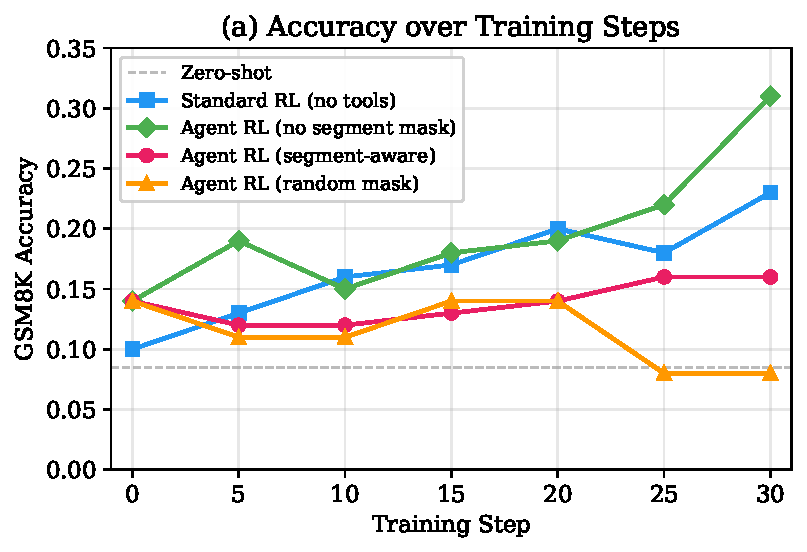
\includegraphics[width=0.95\linewidth]{fig_learning_curves.pdf}
\vspace{-4pt}
\caption{Accuracy over training steps (100-sample periodic evaluation). The zero-shot baseline (8.5\%) is shown as a dashed line. Standard RL and Agent RL without segment masking show steady improvement, while segment-aware Agent RL improves slowly and random masking degrades after step 20.}
\label{fig:learning}
\end{figure}

Standard RL and Agent RL without segment masking show steady improvement, reaching 23\% and 31\% respectively on 100-sample periodic evaluations at step~30. The no-segment variant shows the strongest late-stage improvement (0.22$\to$0.31 from step 25 to 30), suggesting that training on observation tokens accelerates learning in later stages. Agent RL with segment-aware masking improves slowly (14\%$\to$16\%), and random masking degrades after step 20 (14\%$\to$8\%).

\begin{figure}[h]
\centering
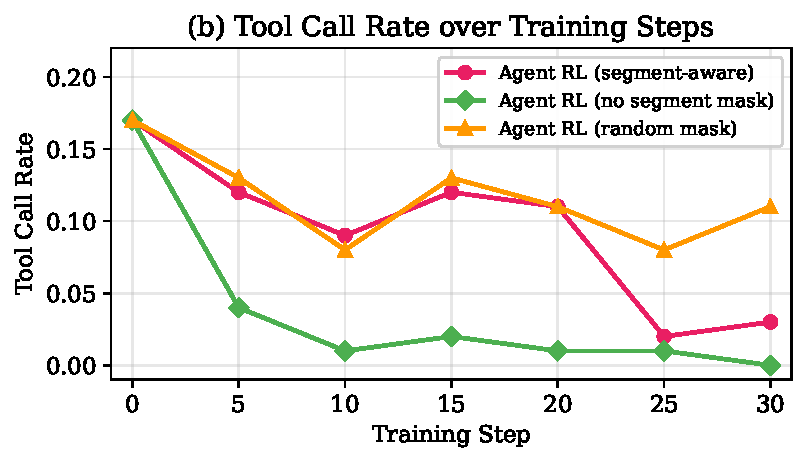
\includegraphics[width=0.95\linewidth]{fig_tool_rate.pdf}
\vspace{-4pt}
\caption{Tool call rate over training steps. All agent RL variants show decreasing tool usage, indicating the model learns to answer directly rather than using tools.}
\label{fig:toolrate}
\end{figure}

\paragraph{Tool call rate decreases with training.}
As shown in Figure~\ref{fig:toolrate}, across all agent RL variants the tool call rate \emph{decreases} over training (from $\sim$17\% to $<$7\%). The model learns to answer directly rather than using tools, as correct tool-free answers receive the same reward. This echoes findings in AR agent RL where tool-use reward shaping is often needed to prevent tool abandonment~\citep{wang2025ragen}.

\begin{figure}[h]
\centering
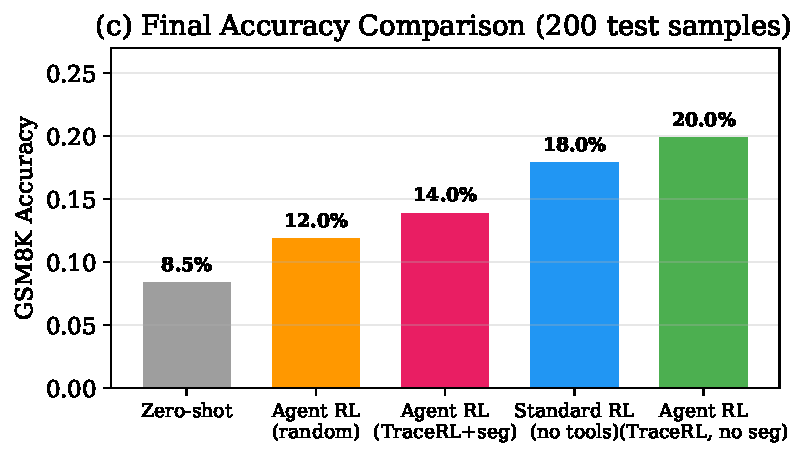
\includegraphics[width=0.95\linewidth]{fig_bar_comparison.pdf}
\vspace{-4pt}
\caption{Final accuracy comparison across all methods (200 test samples). Agent RL without segment masking achieves the highest accuracy among agent variants, surpassing standard RL.}
\label{fig:bar}
\end{figure}

\subsection{Analysis}

\paragraph{Why does segment masking hurt?}
We hypothesize two mechanisms: (1)~observation tokens contain numerical values that teach the model output format and arithmetic patterns, providing a form of ``free supervision''; (2)~segment-aware masking reduces the effective training signal per step (fewer trainable tokens), leading to slower convergence. Future work could test a hybrid approach that applies reduced (but non-zero) loss weight to observation tokens.

\paragraph{When would tools help?}
GSM8K's bottleneck is reasoning, not computation. We expect tool access to be more valuable on benchmarks requiring \emph{external knowledge retrieval} (e.g., multi-hop QA with search) or \emph{code execution} for complex calculations where the model cannot reliably compute answers internally.

% ════════════════════════════════════════════════════════════
\section{Conclusion}

We present the first framework for training multi-turn tool-calling agents on diffusion language models. Our approach extends TraceRL with segment-aware masking, cross-turn step-map composition, and turn-by-turn diffusion generation. Experiments on GSM8K with LLaDA-8B demonstrate that: (1)~RL post-training consistently improves dLLMs on math reasoning, (2)~TraceRL provides better credit assignment than random masking in the agent setting, and (3)~contrary to expectations, training on observation tokens can be beneficial. Our results also show that tool access does not universally help---the benefit depends on whether the task bottleneck aligns with what tools can provide. We release our framework as an extension to dLLM-RL to enable future research on dLLM agents.

\paragraph{Limitations.}
Our experiments use a single base (non-instruction-tuned) model, one benchmark, and one tool type. The findings may not generalize to instruction-tuned dLLMs, search-based QA tasks, or code execution tools. The GSM8K evaluation set is relatively small (200 samples), introducing variance in accuracy estimates.

% ════════════════════════════════════════════════════════════

\bibliographystyle{plain}

\begin{thebibliography}{20}

\bibitem{austin2021d3pm}
J.~Austin, D.~Johnson, J.~Ho, D.~Tarlow, and R.~van~den~Berg.
\newblock Structured denoising diffusion models in discrete state-spaces.
\newblock In \emph{NeurIPS}, 2021.

\bibitem{chai2025rlfactory}
J.~Chai et~al.
\newblock RLFactory: A plug-and-play reinforcement learning post-training framework for LLM multi-turn tool-use.
\newblock \emph{arXiv:2509.06980}, 2025.

\bibitem{cobbe2021gsm8k}
K.~Cobbe, V.~Kosaraju, M.~Bavarian, M.~Chen, H.~Jun, L.~Kaiser, M.~Plappert, J.~Tworek, J.~Hilton, R.~Nakano, C.~Hesse, and J.~Schulman.
\newblock Training verifiers to solve math word problems.
\newblock \emph{arXiv:2110.14168}, 2021.

\bibitem{dream2025}
Dream Team.
\newblock Dream: Diffusion rectification and estimation-adaptive models.
\newblock \emph{arXiv}, 2025.

\bibitem{gou2024tora}
Z.~Gou, Z.~Shao, Y.~Gong, Y.~Shen, Y.~Yang, N.~Duan, and W.~Chen.
\newblock ToRA: A tool-integrated reasoning agent for mathematical problem solving.
\newblock In \emph{ICLR}, 2024.

\bibitem{he2022diffusionbert}
Z.~He, T.~Sun, K.~Wang, X.~Huang, and X.~Qiu.
\newblock DiffusionBERT: Improving generative masked language models with diffusion models.
\newblock In \emph{ACL}, 2023.

\bibitem{lou2024mdlm}
A.~Lou, C.~Meng, and S.~Ermon.
\newblock Discrete diffusion modeling by estimating the ratios of the data distribution.
\newblock In \emph{ICML}, 2024.

\bibitem{lou2024sedd}
A.~Lou and S.~Ermon.
\newblock Score entropy discrete diffusion.
\newblock \emph{arXiv}, 2024.

\bibitem{mercury2025}
Mercury Team.
\newblock Mercury: A reasoning-oriented LLM via discrete diffusion.
\newblock \emph{arXiv}, 2025.

\bibitem{nie2025llada}
S.~Nie et~al.
\newblock LLaDA: Large language diffusion with mAsking.
\newblock In \emph{ICLR}, 2025.

\bibitem{qin2023tool}
Y.~Qin, S.~Liang, Y.~Ye, K.~Zhu, L.~Yan, Y.~Lu, Y.~Lin, X.~Cong, X.~Tang, B.~Qian, et~al.
\newblock ToolLLM: Facilitating large language models to master 16000+ real-world APIs.
\newblock In \emph{ICLR}, 2024.

\bibitem{schick2023toolformer}
T.~Schick, J.~Dwivedi-Yu, R.~Dess{\`i}, R.~Raileanu, M.~Lomeli, E.~Hambro, L.~Zettlemoyer, N.~Cancedda, and T.~Scialom.
\newblock Toolformer: Language models can teach themselves to use tools.
\newblock In \emph{NeurIPS}, 2023.

\bibitem{tracerl2025}
TraceRL Team.
\newblock TraceRL: Revolutionizing post-training for diffusion language models via trajectory-aware policy optimization.
\newblock In \emph{ICLR}, 2026.

\bibitem{wang2024mathshepherd}
P.~Wang et~al.
\newblock Math-Shepherd: Verify and reinforce LLMs step-by-step without human annotations.
\newblock In \emph{ACL}, 2024.

\bibitem{wang2025ragen}
Z.~Wang et~al.
\newblock RAGEN: Understanding self-evolution in LLM agents via multi-turn reinforcement learning.
\newblock \emph{arXiv:2504.20073}, 2025.

\bibitem{wei2025webagent}
Z.~Wei et~al.
\newblock WebAgent-R1: Training web agents via end-to-end multi-turn reinforcement learning.
\newblock \emph{arXiv:2505.16421}, 2025.

\bibitem{xi2025agentgym}
Z.~Xi et~al.
\newblock AgentGym-RL: Training LLM agents for long-horizon decision making through multi-turn reinforcement learning.
\newblock \emph{arXiv:2509.08755}, 2025.

\bibitem{xue2025simpletir}
Z.~Xue et~al.
\newblock SimpleTIR: End-to-end reinforcement learning for multi-turn tool-integrated reasoning.
\newblock \emph{arXiv:2509.02479}, 2025.

\end{thebibliography}

\end{document}
